% Options for packages loaded elsewhere
\PassOptionsToPackage{unicode}{hyperref}
\PassOptionsToPackage{hyphens}{url}
\PassOptionsToPackage{dvipsnames,svgnames*,x11names*}{xcolor}
%
\documentclass[
  10pt,
]{article}
\usepackage{lmodern}
\usepackage{amssymb,amsmath}
\usepackage{ifxetex,ifluatex}
\ifnum 0\ifxetex 1\fi\ifluatex 1\fi=0 % if pdftex
  \usepackage[T1]{fontenc}
  \usepackage[utf8]{inputenc}
  \usepackage{textcomp} % provide euro and other symbols
\else % if luatex or xetex
  \usepackage{unicode-math}
  \defaultfontfeatures{Scale=MatchLowercase}
  \defaultfontfeatures[\rmfamily]{Ligatures=TeX,Scale=1}
  \setmainfont[]{DejaVu Serif}
  \setmonofont[]{DejaVu Sans Mono}
\fi
% Use upquote if available, for straight quotes in verbatim environments
\IfFileExists{upquote.sty}{\usepackage{upquote}}{}
\IfFileExists{microtype.sty}{% use microtype if available
  \usepackage[]{microtype}
  \UseMicrotypeSet[protrusion]{basicmath} % disable protrusion for tt fonts
}{}
\makeatletter
\@ifundefined{KOMAClassName}{% if non-KOMA class
  \IfFileExists{parskip.sty}{%
    \usepackage{parskip}
  }{% else
    \setlength{\parindent}{0pt}
    \setlength{\parskip}{6pt plus 2pt minus 1pt}}
}{% if KOMA class
  \KOMAoptions{parskip=half}}
\makeatother
\usepackage{xcolor}
\IfFileExists{xurl.sty}{\usepackage{xurl}}{} % add URL line breaks if available
\IfFileExists{bookmark.sty}{\usepackage{bookmark}}{\usepackage{hyperref}}
\hypersetup{
  colorlinks=true,
  linkcolor=Maroon,
  filecolor=Maroon,
  citecolor=Blue,
  urlcolor=Blue,
  pdfcreator={LaTeX via pandoc}}
\urlstyle{same} % disable monospaced font for URLs
\usepackage[margin=0.6in,landscape]{geometry}
\usepackage{longtable,booktabs}
% Correct order of tables after \paragraph or \subparagraph
\usepackage{etoolbox}
\makeatletter
\patchcmd\longtable{\par}{\if@noskipsec\mbox{}\fi\par}{}{}
\makeatother
% Allow footnotes in longtable head/foot
\IfFileExists{footnotehyper.sty}{\usepackage{footnotehyper}}{\usepackage{footnote}}
\makesavenoteenv{longtable}
\usepackage{graphicx}
\makeatletter
\def\maxwidth{\ifdim\Gin@nat@width>\linewidth\linewidth\else\Gin@nat@width\fi}
\def\maxheight{\ifdim\Gin@nat@height>\textheight\textheight\else\Gin@nat@height\fi}
\makeatother
% Scale images if necessary, so that they will not overflow the page
% margins by default, and it is still possible to overwrite the defaults
% using explicit options in \includegraphics[width, height, ...]{}
\setkeys{Gin}{width=\maxwidth,height=\maxheight,keepaspectratio}
% Set default figure placement to htbp
\makeatletter
\def\fps@figure{htbp}
\makeatother
\setlength{\emergencystretch}{3em} % prevent overfull lines
\providecommand{\tightlist}{%
  \setlength{\itemsep}{0pt}\setlength{\parskip}{0pt}}
\setcounter{secnumdepth}{-\maxdimen} % remove section numbering
\renewcommand{\arraystretch}{1.6}

\author{}
\date{}

\begin{document}

\hypertarget{stage-1.0-range-table-targeting-powered-ascent-ballistic-arc}{%
\section{Stage 1.0 --- Range Table Targeting (Powered Ascent + Ballistic
Arc)}\label{stage-1.0-range-table-targeting-powered-ascent-ballistic-arc}}

\textbf{Era:} Redstone/Mercury-Redstone class, \textasciitilde1961
(fictional program). \textbf{Prerequisite:} Phase 0 (all four drills).
\textbf{Depends on:} 0.0, 0.1 (slide rule, table interpolation)
directly; 0.3 (triangle solving) indirectly, for the same ``expect more
than one valid answer'' habit.

This version deliberately simplifies two things --- a constant Isp and a
given, un-derived loss budget --- to keep the first Stage 1 problem to
about half an hour. For the harder, more complete version of this same
ascent (where both of those are derived rather than assumed), see
\textbf{1.1} (liftoff sanity check + gravity-turn loss,
first-principles) and \textbf{1.2} (non-constant Isp, full afternoon).

\hypertarget{narrative-frame}{%
\subsection{Narrative frame}\label{narrative-frame}}

You're the flight dynamics engineer for \textbf{Project Arrowhead}, a
fictional 1961 suborbital test program flying the \textbf{Redwing-3}
booster out of a fictional coastal range. Range Safety has assigned
tomorrow's flight an impact zone centered \textbf{210.0 nautical miles}
downrange of the pad, inside a larger safety corridor. Your job: using
the vehicle's known performance and a burnout altitude fixed by the
guidance program, build the range table for this vehicle and tell the
pad crew what burnout flight path angle(s) will put the impact where
Range Safety wants it --- and confirm there's more than one way to get
there.

\hypertarget{given-data}{%
\subsection{Given data}\label{given-data}}

\textbf{Vehicle performance (powered ascent):} - Gross liftoff weight,
W₀ = 55,000 lbf - Propellant weight burned to cutoff, Wₚ = 40,000 lbf -
Effective specific impulse, Iₛₚ = 235 s (treated as constant --- real
engines vary Iₛₚ with altitude, but a single effective value is the
period-standard simplification for a first-pass performance estimate;
see 1.2 for the non-constant version) - Burn time, t\_b = 143 s -
Gravity + drag loss allowance, Δv\_losses = 3540 ft/s (derived in 1.1
from a first-principles gravity-turn/drag integration --- treat it as a
given here, the way a real FDO would receive it from the trajectory
design group, having not run that study themselves)

\textbf{Ballistic arc:} - Burnout altitude, h\_bo = 100,000 ft (fixed by
the guidance program, independent of flight path angle --- this matches
the altitude 1.1's gravity-turn study actually converges to, which is
not a coincidence: the pitch program in 1.1 was designed to hit it) -
Standard gravity, g = 32.174 ft/s² (treated as constant with altitude
--- valid at these altitudes to within a few percent, and consistent
with the flat, non-rotating Earth model used throughout this problem) -
Assume impact at sea level (flat, non-rotating Earth --- no curvature
correction at this range; that correction is flagged as a natural
extension for a later, longer-range stage)

\textbf{Target:} impact range = 210.0 nautical miles from the pad (1 nm
= 6076.12 ft)

\hypertarget{authentic-method-reference-material}{%
\subsection{Authentic method + reference
material}\label{authentic-method-reference-material}}

\textbf{Powered ascent --- Tsiolkovsky rocket equation} (Tsiolkovsky,
1903; in active use by every rocket engineer of this era):

\begin{verbatim}
Δv_ideal = c · ln(W₀/W₁)          c = Iₛₚ · g₀
V_bo = Δv_ideal − Δv_losses
\end{verbatim}

where W₁ = W₀ − Wₚ is burnout weight.

\textbf{Ballistic arc --- flat-Earth, uniform-gravity vacuum
trajectory.} This is the same mathematics behind WWII- and V2-era
artillery/rocket range tables, which the Redstone program inherited
directly through von Braun's team. It is \emph{not} the full
spherical-Earth treatment (Bate, Mueller \& White, Ch. 4, ``Ballistic
Missile Trajectories,'' which treats the free-flight arc as a conic with
one focus at Earth's center) --- that's intentionally saved for a later,
longer-range stage, since Stage 1 is scoped to stay out of orbital
mechanics. At suborbital ranges like this one, the flat-Earth form is an
accurate and period-appropriate simplification, not a shortcut that
sacrifices authenticity.

With burnout velocity V\_bo at flight path angle γ (measured above local
horizontal) and altitude h\_bo:

\begin{verbatim}
v_y0 = V_bo · sin(γ)        v_x0 = V_bo · cos(γ)

t_impact = [v_y0 + √(v_y0² + 2·g·h_bo)] / g

R = v_x0 · t_impact

h_apex = h_bo + v_y0² / (2g)
\end{verbatim}

\textbf{The graphical range-table method:} rather than solving R(γ) =
210.0 nm directly (it's not algebraically clean to invert), compute R
for a spread of γ values, sketch R vs.~γ by hand, and read the answer(s)
off the curve. This is exactly how real range tables were built and used
operationally --- a chart, not an equation to invert on demand. Expect
the curve to be non-monotonic near its peak, which means \textbf{two}
valid flight path angles can produce the same range: a flatter,
faster-arriving trajectory and a more lofted one. Same ambiguity in
spirit as the SSA triangle case in 0.3 --- don't be surprised by it, and
don't discard one root as ``wrong.''

\hypertarget{worksheet}{%
\subsection{Worksheet}\label{worksheet}}

\textbf{Part A --- Burnout velocity}

\begin{longtable}[]{@{}ll@{}}
\toprule
Quantity & Value\tabularnewline
\midrule
\endhead
W₁ = W₀ − Wₚ &\tabularnewline
c = Iₛₚ · g₀ &\tabularnewline
W₀/W₁ &\tabularnewline
ln(W₀/W₁) &\tabularnewline
Δv\_ideal = c·ln(W₀/W₁) &\tabularnewline
V\_bo = Δv\_ideal − Δv\_losses &\tabularnewline
\bottomrule
\end{longtable}

\textbf{Part B --- Range table.} Fill in for each γ. Carry v\_y0²
through in full (you'll reuse it for the apex altitude too --- don't
recompute).

\begin{longtable}[]{@{}llllllllll@{}}
\toprule
γ & sin γ & cos γ & v\_y0 & v\_x0 & v\_y0² & t\_impact (s) & R (ft) & R
(nm) & h\_apex (ft)\tabularnewline
\midrule
\endhead
30° & & & & & & & & &\tabularnewline
35° & & & & & & & & &\tabularnewline
40° & & & & & & & & &\tabularnewline
45° & & & & & & & & &\tabularnewline
50° & & & & & & & & &\tabularnewline
55° & & & & & & & & &\tabularnewline
\bottomrule
\end{longtable}

\textbf{Part C --- Graphical solution.} Plot R (nm, vertical axis) vs.~γ
(horizontal axis, 30°--55°) on the grid below using your six points from
Part B. Draw a horizontal line at R = 210.0 nm and read off both
crossings.

\begin{figure}
\centering
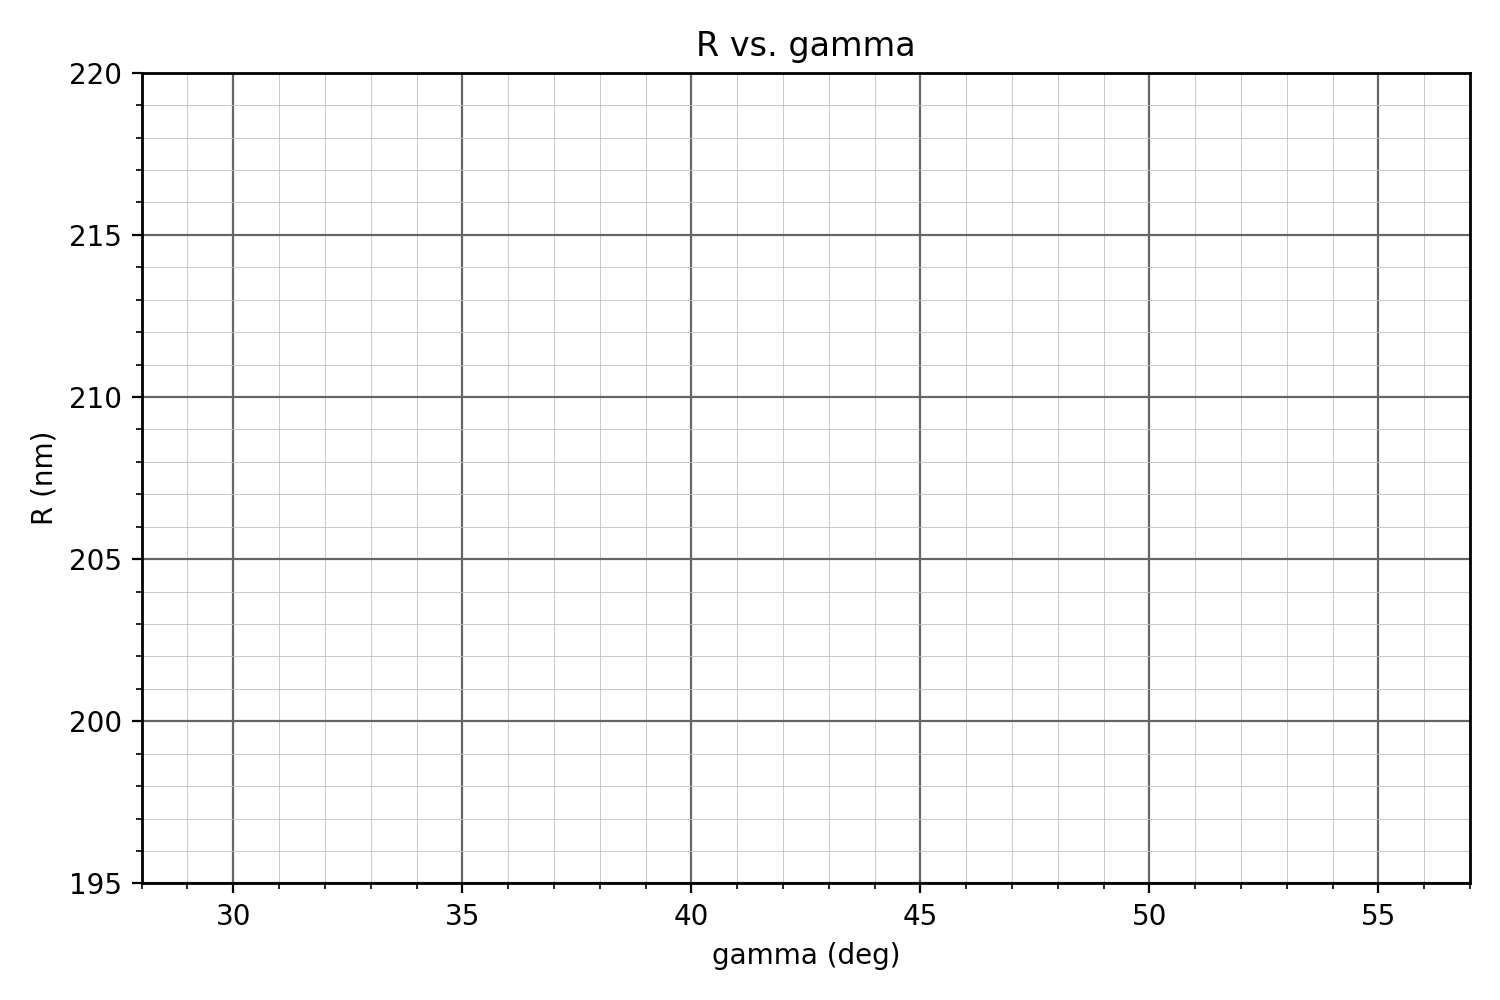
\includegraphics{01-range-table-targeting-worksheet-grid_1.png}
\caption{R vs.~gamma}
\end{figure}

Low-angle solution: γ = \_\_\_\_\_\_\_\_\_\_° High-angle solution: γ =
\_\_\_\_\_\_\_\_\_\_°

\end{document}
